\subsubsection{Surface Science } \index{Tautz, Stefan}

\paragraph{Research Team}
Stefan Tautz (Professor), Torsten Balster (Research Associate),
Stina Henze (Postdoctoral Fellow), Serguei
Soubatch (Research Associate), Ruslan Temirov (PhD Student)\\

In surface and interface science, physical and chemical processes
at the boundaries between different phases of condensed matter,
e.g.~solid-liquid, solid-gas or solid-solid interfaces, are
investigated. Nature abounds with such interfaces. They impart
both structure and function to the material world, including
living matter. Therefore, surface science is an interdisciplinary
research field, involving physicists, chemists and - more recently
- biologists alike.

The surface science group at IUB specializes in the investigation
of bonding, structure and function of molecular adsorbate layers
on solid surfaces. The surface adsorption of complex molecules is
an important topic in many applied research fields, including
electronics, sensor technology, catalysis, and adhesive
technology. A special focus of our work are the interfaces of
organic semiconductors with metals and insulators. Such
interfaces play a crucial role in the emerging fields of organic
and molecular electronics, which are generally perceived as two
of the key technologies for the future of electronics.

\paragraph{Highlights}
In 2006, we have worked along three lines of investigation.
First, we have completed a range of experiments on structural
organization in complex molecular architectures on surfaces
\cite{Tautz6, Tautz7}, second, we have continued our efforts to
improve the understanding of the bonding of $\pi$-conjugated
molecules on surfaces \cite{Tautz1,Tautz4,Tautz5,Tautz8,Tautz10},
and third, we have extended our spectroscopic and microscopic
work on highly ordered organic interface layers to single molecule
transport experiments \cite{Tautz9}.

In the spirit ``Function through Architecture'', complex molecular
architectures are a promising pathway to obtain functional
materials for applications in catalysis, sensing and information
processing. This is true for 3D bulk materials as well as 2D
molecular layers at surfaces. Understanding the structural
organization in these materials is a key problem. We have
approached this problem for two classes of molecules: The
amino-acid L-DOPA [3-(3,4-Dihydroxyphenyl)alanine] is a
multi-functional and chiral molecule and as such a representative
for chiral organization at surfaces, while the molecule DH4T
[$\alpha$,$\omega$-dihexyl-quaterthiophene] is a mesogenic
molecule, which due to their internal flexibility allow the
formation of liquid crystalline phases. For the former, we have --
in the framework of a diploma thesis in cooperation with the
University Bremen -- suggested a structural model for the ordered
surface phase on Au(110) \cite{Tautz7}, while for the latter we
have investigated the structural organization in the sway of three
competing factors, namely molecule-substrate interaction,
intermolecular interactions and molecular mesogenicity, and indeed
found a reversible order-to-disorder phase transition on Ag(111)
\cite{Tautz6}. Together with our ongoing efforts at the European
Synchrotron Radiation Facility at Grenoble, these will form the
basis of a new project entitled: ``Complex molecular architectures
at surfaces: From quantitative structures to mechanisms of
structural organization''.

Concerning the bonding of $\pi$-conjugated molecules on metal
surfaces \cite{Tautz1,Tautz4,Tautz5,Tautz8,Tautz10}, the most
notable result is perhaps our discovery of a very large electron
dispersion (and hence delocalization) in a molecular PTCDA film
close to a metal surface (cf.~Fig.~\ref{fig:profTautz}). This
finding is reported in a \textsl{Letter to Nature} \cite{Tautz5}.
Electronic band dispersion in molecular solids is currently a hot
topic, because dispersion measurements promise to shed some light
on charge carrier transport mechanisms. In the present case, a
much stronger dispersion than expected for the molecular film on
its own is observed close to the metal. Clearly, the proximity of
the metal plays an important role, but the results show that the
molecules are also crucially involved in the corresponding
electron state at the interface of the two. Through their complex
chemical interaction, metal and molecule conspire to form a thin
interface layer with new and surprising properties, neither purely
metallic nor purely molecular. Both partners thus give up part of
their identity to form something new. This is interesting from the
materials science point of view, since metal-organic interfaces
are a basic building blocks of metal-organic hybrid materials. The
present results thus indicate that novel materials with
interesting electronic and transport properties may be created if
advantage is taken of the new properties emerging at hybrid
interfaces.

The findings also have fundamental implications. The experiment
is the latest in a series of experiments which force us to
reconsider our perceived understanding of the interaction of
semiconducting molecules with metal surfaces. Originally, it had
been thought that there would be little or no chemical
interaction present, but this has clearly been disproved now by
this and other recent work.

Finally, we have developed a new approach to single-molecule
transport experiments \cite{Tautz9}. It is based on perfectly
ordered, epitaxial layers of molecules on a single crystalline
metal substrate. Such layers offer the advantage that molecules
are adsorbed in well-defined adsorption sites; the electronic
properties of the metal-molecule contact can therefore be
characterized by a wide range of spectroscopic experiments. This
new approach thus addresses the most difficult challenge of single
molecule transport experiments, namely the problem of structural
definition and control at the contacts. In our experiments, both
are realized to a very high degree. First results have been
submitted for publication. In future, we will develop these
experiments further. \nocite{Tautz2,Tautz3}
\begin{figure}[ht]
  \begin{center}
    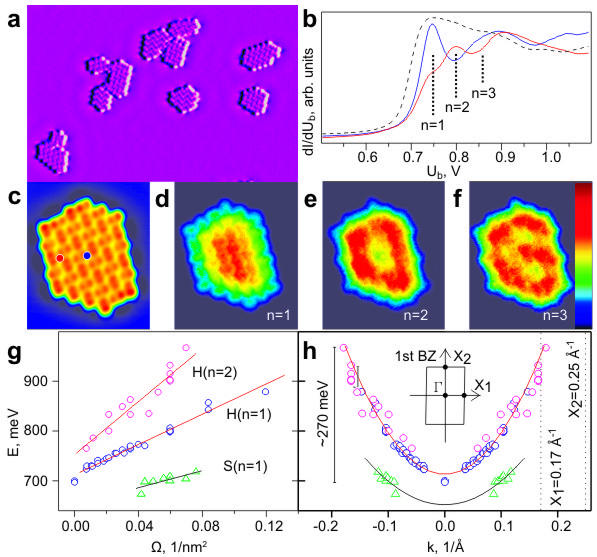
\includegraphics[width=\hsize]{Tautz/profTautz-fig1.jpg}
    \mycaption{Free-electron-like 2D band state of PTCDA/Ag(111), measured by confining it to nanoscale molecular islands.}\label{fig:profTautz}
   \end{center}
\end{figure}

\paragraph{Organization}
\begin{enumerate}
\item Invitation to organize the 383.~WEH Heraeus Seminar.
\end{enumerate}

\paragraph{Collaborations}
\begin{enumerate}
\item {\sl Universit\"at Bonn} \\ Prof. Dr. M. Sokolowski \\ NIXSW
experiments on molecular films
 \item {\sl Technische Universit\"at
Ilmenau} \\ Dr. M. Eremtchenko, Prof. Dr. J.A. Schaefer \\
Vibrational properties of silicon surfaces \item {\sl
Universit\"at W\"urzburg} \\ Prof. Dr. E. Umbach \\ Phaser of
organic adsorbates on metal surfaces
\item {\sl Link\"oping University} \\ Prof. Dr. M Fahlmann\\
Resonant
photoemission experiments on molecular films \item {\sl Lund University} \\
Prof. Dr. S. Sorensen \\ Resonant photoemission experiments on
molecular films
\item {\sl Universit\"at Bremen} \\ Prof. Dr. B. Jastorff \\
Adsorption of amino acids on solid surfaces \item {\sl Universit\"at Bremen} \\
Prof. Dr. Th. Frauenheim \\ Inealstic tunnelling and quantum
transport through molecules  \item {\sl Universit\"at Osnabr\"uck}
\\ Prof. Dr. M. Rohlfing \\ Structure and properties of molecular
adsorbates  \item
{\sl International University Bremen} \\ Prof. Dr. V. Wagner\\
Organic and molecular electronics  \\ Prof. Dr. A. Materny\\
Raman-excitation spectroscopy on molecular films
\item {\sl Forschungszentrum J\"ulich} \\ Prof. Dr. H. Ibach\\
Vibrational properties of silicon carbide surfaces
\end{enumerate}

\paragraph{Grants}
% list the running grants in 2005, if none have been received, please delete this
% subsection.
\begin{enumerate}
\item Funded by DFG, \emph{Local vibronic and
geometric structure of large organic adsorbates: New experimental
approaches to chemisorption by STM-IETS and NIXSW} (April 2005 -
March 2008)
\end{enumerate}

\paragraph{Other Support Grants}
% list the running grants in 2005, if none have been received, please delete this
% subsection.
\begin{enumerate}
\item {Wenner-Gren Foundation} Post-doctoral grant for Dr. S. K.
M. Henze.

\item {European Synchrotron Radiation Facility, Grenoble}:
``Interplay between lateral and vertical adsorption structure,
studied by NIXSW on PTCDA monolayers adsorbed on Ag(100), Ag(110)
and Ag(111) (SI-1451)'' (in cooperation with Prof. Dr. M.
Sokolowski, Universit\"at Bonn).

\item {MAX-Lab, Lund, Sweden}: ``Resonant photoemission for
monolayers and multilayers of PTCDA on Ag(111): life-times of
unoccupied valence states determined by the core-hole clock
technique.'' (in cooperation with Prof. Dr. S. Sorenson, Lund
University, and Prof. Dr. M. Fahlmann, Link\"oping University).

\item {Wilhelm und Else Heraeus Foundation} Grant for organization
of the 383.~WEH Seminar on the ``Physics of Highly Ordered Organic
Interface Layers'', to be held in Bad Honnef, January 22-24, 2007
(in cooperation with Prof. Dr. M. Sokolowski, Universit�t Bonn).
\end{enumerate}

\paragraph{Awards, Prizes}
% list the grants you have received in 2005, if none have been received, please delete this
% subsection.
\begin{enumerate}
\item Invitation to write a book chapter for American Scientific
Publishers.
\end{enumerate}
